\documentclass[ngerman]{scrartcl}
\usepackage{babel}
\usepackage{fontspec}
\setmainfont{Open Sans}[
  BoldFont={Open Sans Bold},
  ItalicFont={Open Sans Italic}]
\setsansfont{Open Sans}[
  BoldFont={Open Sans Bold},
  ItalicFont={Open Sans Italic}]
\setmonofont{Menlo}
\usepackage{xcolor}
\usepackage{soul}
\usepackage{enumitem}
\usepackage{listings}
\usepackage{graphicx}
\lstset{basicstyle=\ttfamily,escapeinside=||}


% nice tables
\usepackage{booktabs}
\newcommand{\tablespacing}[1]{\renewcommand{\arraystretch}{#1}}

\title{Einführung in den Compilerbau}
\date{Wintersemester 2018-2019}
\author{Andreas Koch}

\begin{document}
  \maketitle
  \tableofcontents
  \newpage
  
  %\KOMAoptions{twocolumn}
  
  \section{Organisatorisches}
   
  \subsection{Grundlage der Vorlesung}
   
  Die Vorlesung basiert \hl{fast vollständig} auf \emph{Programming Language Processors in Java}\footnote{von David Watt und Deryck Brown, Prentice-Hall 2000}. Auszugsweise noch weiteres Material, z.\ B.\ zum ANTLR-Parsergenerator.
  
  \subsection{Übersichtswerk}
  
  Einen guten allgemeinen Überblick, aber im Detail mit anderen Schwerpunkten als diese Vorlesung, bietet \emph{Compilers, 2. Auflage}\footnote{Von Aho, Sethi, Ullmann, Lam, Addison-Wesley 2006. Auch auf Deutsch verfügbar.}.
   
  \subsection{Aufbau der Veranstaltung}
  
  Diese Veranstaltung ist logisch in mehrere Teile gegliedert.
  
  \begin{description}
    \item[Front-End\footnotemark] Übersicht, ca.\ 3 Wochen.
    \begin{itemize}
      \item Lexing und Parsing,
      \item Zwischendarstellungen.
    \end{itemize}
    \item[Middle-End] Übersicht, ca.\ 2 Wochen.
    \begin{itemize}
      \item Semantische- und Kontextanalyse.
    \end{itemize}
    \item[Back-End] Übersicht, ca.\ 4 Wochen.
    \begin{itemize}
      \item Laufzeitorganisation,
      \item Code-Erzeugung.
    \end{itemize}
    \item[Front-End-Generatoren] Verwendung, ca.\ 2--3 Wochen.
    \item[Java Virtuelle Maschine] ca.\ 1--2 Wochen.
  \end{description}
  \footnotetext{Die ersten drei Teile der Veranstaltung richten sich an die Veranstaltungen \emph{IMT3052} von Ivar Farup, Universität Grøvik, Norwegen; und \emph{Vertalerbouw} von Theu Ruys, Universität Twente, Niederlande.}
  
  \section{Einleitung}
  
  \subsection{Compiler}
  
  Ein Compiler ist eine Schnittstelle zwischen \emph{Mensch} und \emph{Maschine}. Er übersetzt von einer Programmiersprache (Menschenlesbar) in eine Maschinensprache (maschinenlesbar).
  
  \begin{description}
    \item[Programmiersprache] Gut für Menschen lesbar. Beispiele für Programmiersprachen sind:
    \begin{itemize}
      \item Smalltalk, 
      \item Java, 
      \item C++.
    \end{itemize}
    \item[Maschinensprache] Getrimmt auf
    \begin{itemize}
      \item Ausführungsgeschwindigkeit,
      \item Preis pro Chip, Fläche,
      \item Energieverbrauch,
      \item (nur selten) leichte Programmierbarkeit.
    \end{itemize}
  \end{description}
  
  \subsection{Auswirkung von Compilern}
  Mit den Eigenschaften entscheidet ein Compiler über die dem Nutzer zugängliche Rechenleistung. Durch gewisse Abwägungen kann ein Compiler ein Programm so kompilieren, dass es am schnellsten läuft oder dass der Resultierende Code an kleinsten ist.
  
  \begin{table*}[h]
  \centering
  \tablespacing{1.2}
  \begin{tabular}{@{}lp{.5cm}lp{.5cm}l@{}}
    \toprule
      Compiler && Ausführungszeit && Programmgröße\\
      \midrule
        GCC 3.3.6 && 7,5\,ms && 13\,KB\\
        ICC 9.0 && 6,5\,ms && 511\,KB\\
      \bottomrule
  \end{tabular}
  \caption{Bildkompression auf Dothan CPU, 2\,GHz}
  \end{table*}

  \subsection{Programmiersprachen}

\begin{description}
\item[Hohe Ebene] Smalltalk, Java, C++. Beispiel:
\begin{lstlisting}
let
  var i : Integer;
in
  i := i + 1;
\end{lstlisting}
\item[Mittlere Ebene] Assembly
\begin{lstlisting}
LOAD  |\hl{R1}|, (i)
LOADI |\hl{R2}|, 1
ADD   |\hl{R1}|, R1, R2
STORE R1, (i)
\end{lstlisting}
\item[Niedrige Ebene] Machinensprache
\begin{lstlisting}
01100001|\hl{00000110}|
0111001001000001
1011000100010010
10010001|\hl{00000110}|
\end{lstlisting}
\end{description}

\subsection{Abstraktionsebenen}

Auf den unteren Ebenen werden die Beschreibungen immer feiner, da man näher an der Zielmaschine (Hardware) arbeitet.

Der Compiler ist dafür zuständig, Details hinzuzufügen. In den obenstehenden Codebeispielen musste der Compiler unter anderem Register wählen, in denen die Werte währen dem Programmablauf zwischengespeichert werden. Außerdem musste die Adresse der Variable \verb|i|, hinzugefügt werden, wobei hier \verb|00000110| verwendet wurde.

Diese Details werden mithilfe von verschiedensten Algorithmen ergänzt, welche die \hl{Programmeigeschaften Analysieren} und durch die \hl{Synthese von Details} die Beschreibung Verfeinern.

\section{Zielmaschine}

\subsection{Auswirkungen der Zielmaschine}

\begin{figure}
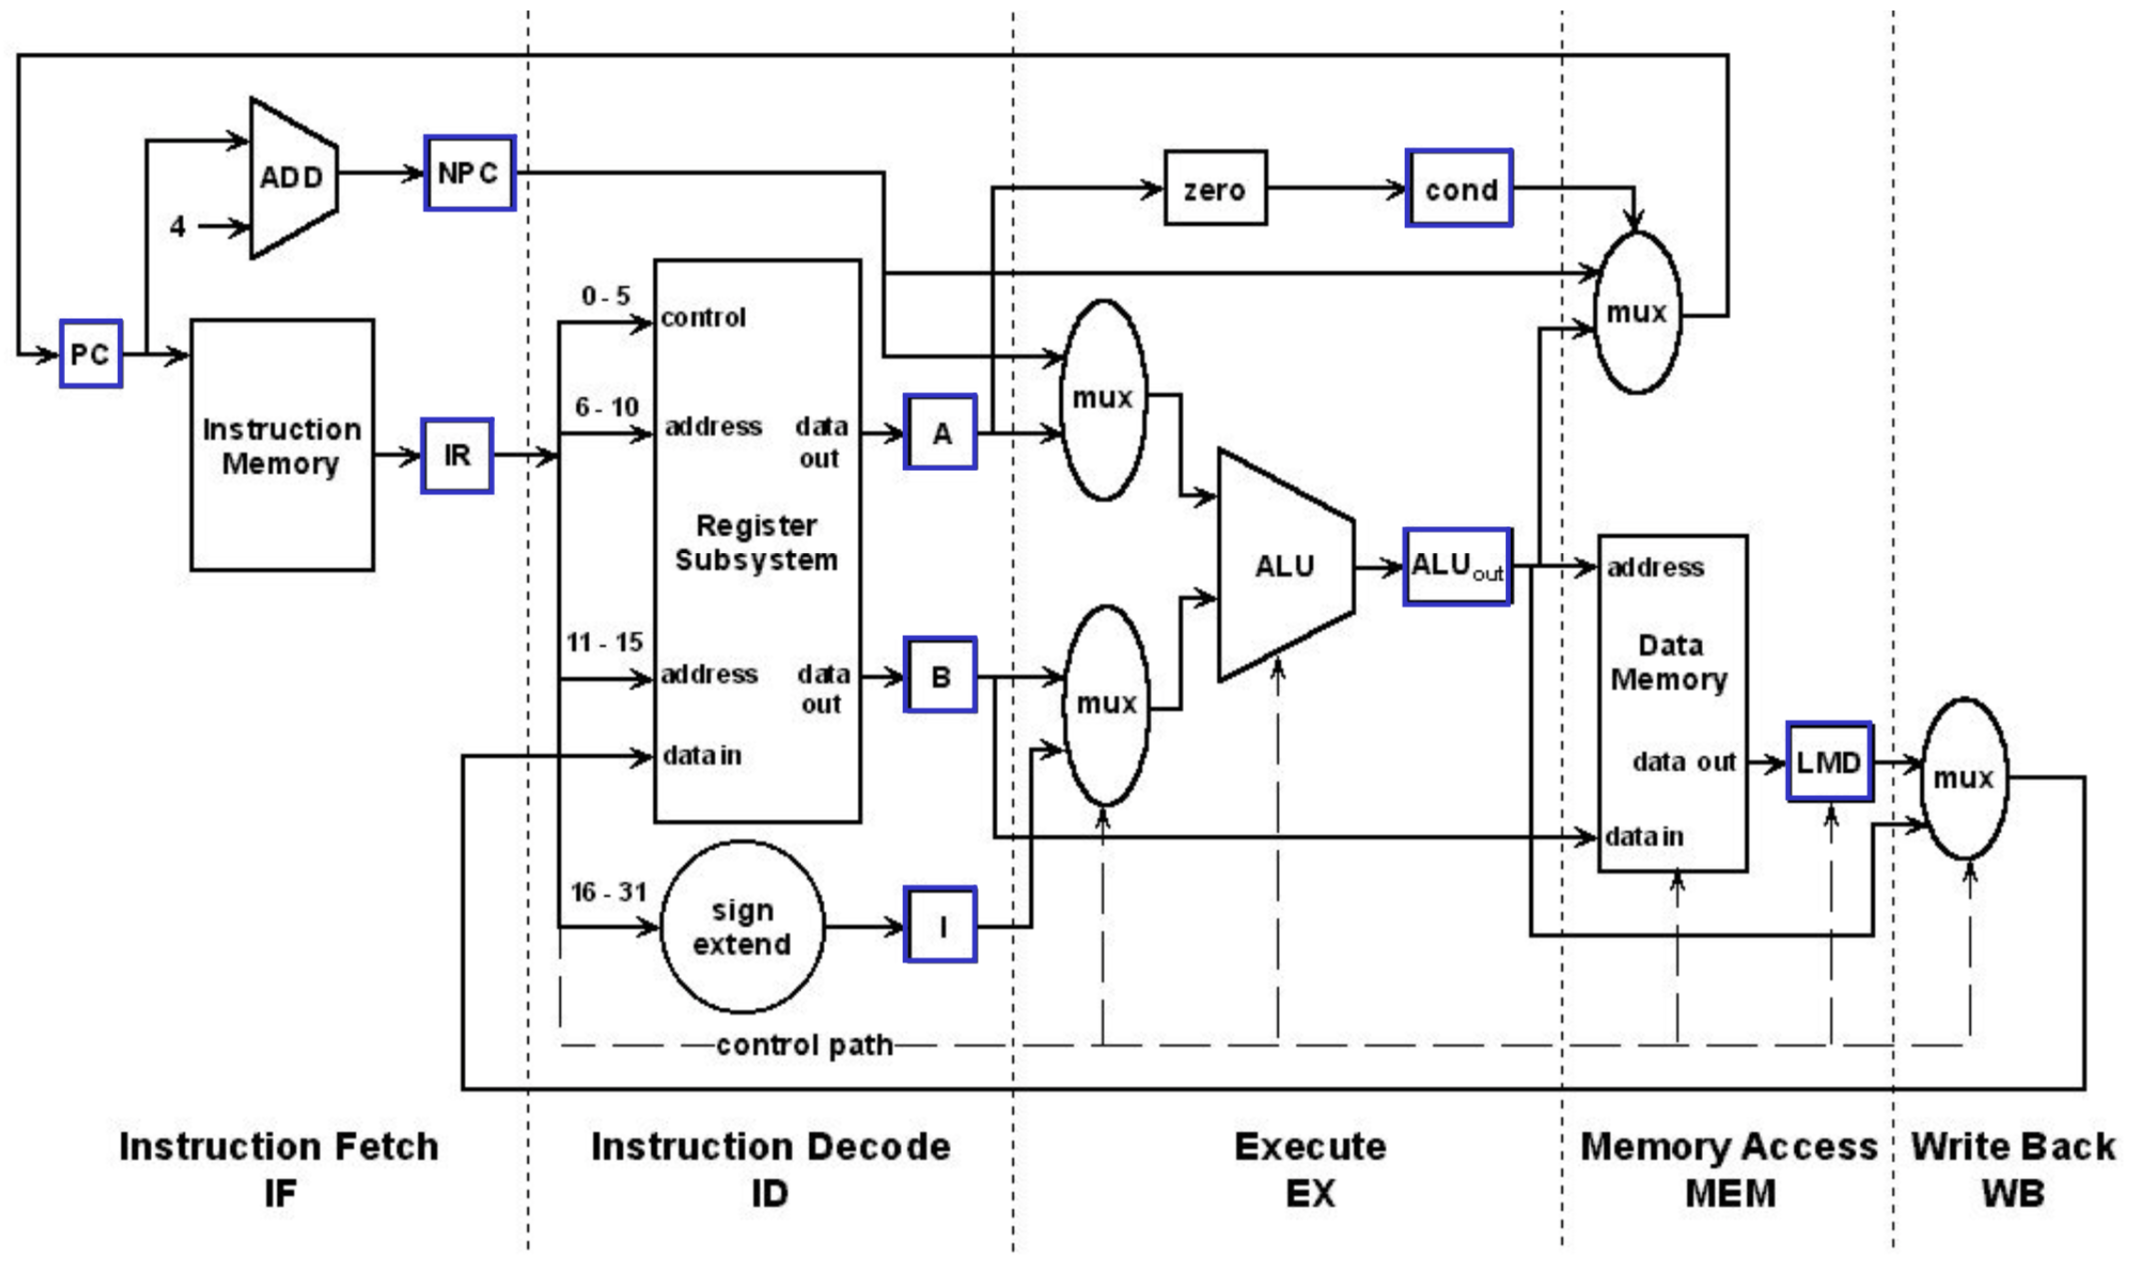
\includegraphics[width=\textwidth]{media/dlx}
\caption{Die DLX RISC Prozessorarchitektur}
\end{figure}
\begin{figure}
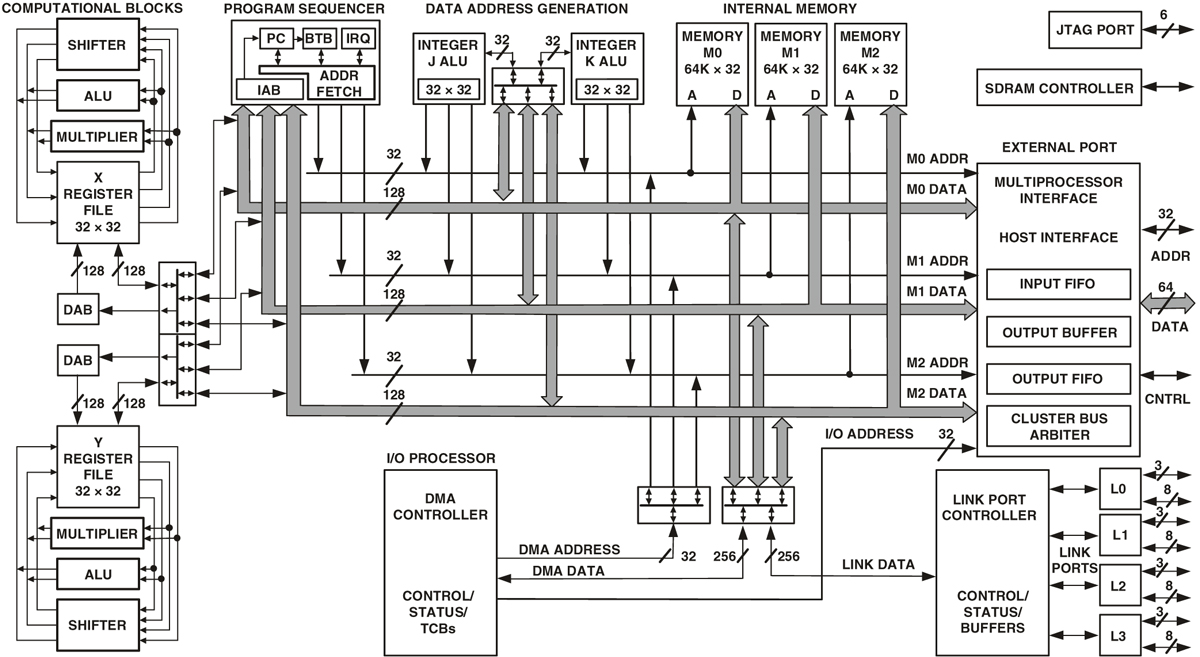
\includegraphics[width=\textwidth]{media/tigersharc}
\caption{Analog Devices TigerSHARC}
\end{figure}

Die Zielmaschine hat einen Einfluss auf die Architektur des Compilers. So basiert zum Beispiel die DLX Architektur von John Hennessy und David Patterson auf der MIPS Architektur, und ist nur leicht verändert um diese zu modernisieren. Damit ist es sehr einfach, einen Compiler zu bauen, der für diese Architektur Code generiert.

Etwas komplizierter wird es mit der \emph{TigerSHARC} Architektur von Analog Devices. Dies ist ein Beispiel für ein DSP, also \emph{Digital Signalling Processor}. Es gibt hier zwei \emph{Computational Blocks}, damit parallel Rechnungen ausgeführt werden können. Diese können aber nicht kommunizieren, also muss der Compiler drauf achten, dass auf die Register nur von dem jeweiligen Block aus zugegriffen werden können. Außerdem besitzt diese Architektur separate Rechenblocks, um Adressen zu bestimmen. Ein Compiler für diese Architektur muss also wissen, wie die Architektur aufgebaut ist, um sie effizient zu nutzen.

Am problematischsten wird das aber erst bei extremen Architekturen wie der des IBM/Sony \emph{Cell} Prozessors. Hierbei handelt es sich um eine sehr gewagte, und wie sich leider heraus



\end{document}










